\documentclass[12pt]{article}
\usepackage[OT4]{fontenc}
\usepackage[polish]{babel}
\usepackage[legalpaper, margin=2cm]{geometry}
\usepackage{mathtools}
\usepackage{float}
\usepackage{hyperref}
\usepackage{svg}
\usepackage{graphicx}
\usepackage{placeins}
\usepackage{chngcntr}

\newif\ifpokazsekcjaszesc
\pokazsekcjaszesctrue

\title{Sprawozdanie z drugiej połowy projektu\\
Przedmiotu "Wizualizacja Danych"}
\author{Grupa Pon 14:15 - 17:00, \\zespół 4 - Jan Domański, Maciej Kurzydłowski, Jan Machowski}
\date{sem. 26L}

\begin{document}
\maketitle
\tableofcontents
\newpage

% Proponowana struktura rozdziału
% 1. Źródło danych
% 2. Opis zbioru i istotnych pojęć - o czym jest, pojęcia z nim związane, kolumny, czy dane są kateg / liczb/
% 3. Wizualizacja + krótki opis co pokazuje
% 4. Wnioski


% \subsubsection{}
% \begin{figure}[H]
%     \includegraphics[width=\textwidth]{phts/}
%     \caption{}
% \end{figure}


\section{Trzęsienia ziemi na świecie}

Przygotowane przez: Maciej Kurzydłowski

\subsection{Źródło danych}
\href{https://www.usgs.gov/programs/earthquake-hazards}{USGS - Earthquake Hazards - API}\\
\url{https://www.usgs.gov/programs/earthquake-hazards}

\subsection{Opis zbioru i istotnych pojęć}
\begin{itemize}
    \item Dane zostały pobrane przez API. W ramach wizualizacji zostało pobranych 3240855 rekordów trzęsień ziemi z całego świata;
    \item Dane zostały zebrane w przedziale 2000 - 2026 roku;
    \item Dane zawierały informacje o czasie, miejscu, głębokości, magnitudzie, etc. dla każdego trzęsienia ziemi;
    \item Wielkość pliku z danymi wynosiła około 500 MB, co może być problematyczne przy odtwarzaniu wizualizacji.
\end{itemize}

\newpage


\subsubsection{Trzęsienia ziemi wokół świata}
\begin{figure}[H]
    \centering
    
\includegraphics[width=\textwidth]{phts/1/png/1.png}
    \caption{Rozmieszczenie trzęsień ziemi na mapie świata.}
\end{figure}

Mapa światowa pokazuje, że trzęsienia ziemi koncentrują się głównie wzdłuż granic płyt tektonicznych. Największe skupiska widać wokół Pacyfiku, ale podobne pasma aktywności pojawiają się także w rejonie Alp, Indonezji i Ameryki Południowej.

\subsubsection{Wizualizacja sejsmiczności w czasie}
\begin{figure}[H]
    \centering
    
\includegraphics[width=\textwidth]{phts/1/png/2.png}
    \caption{Animacja sejsmiczności na mapie świata dla kolejnych lat. (Tylko pierwsza klatka)}
\end{figure}

Animacja pokazuje w miarę równe rozłożenie trzęsień ziemi w czasie, bez znacznych zauważalnych zdarzeń.

\subsubsection{Gęstość trzęsień ziemi o wysokiej magnitudzie}
\begin{figure}[H]
    \centering
    
\includegraphics[width=\textwidth]{phts/1/png/3.png}
    \caption{Mapa gęstości trzęsień ziemi o magnitudzie powyżej 5.}
\end{figure}

Mapa pokazuje znaczącą przewagę ilości trzęsień ziemi w rejonach Pacyfiku, w porównaniu do innych płyt tektonicznych.

\subsubsection{Liczba trzęsień ziemi w czasie}
\begin{figure}[H]
    \centering
    
\includegraphics[width=\textwidth]{phts/1/png/4.png}
    \caption{Liczba trzęsień ziemi w czasie.}
\end{figure}

Liczba trzęsień ziemi jest mało stabilna w czasie, z zauważalnymi okresami wzrostów aktywności sejsmicznej. Spadek liczby trzesień na końcu wykresu jest spowodowany dzieleniem przedziału na kubki o długości 1 miesiąca - ostatni miesiąc nie jest w pełni udokumentowany.

\subsection{Wizualizacje zbioru}
\subsubsection{Rozkład magnitud trzęsień ziemi}
\begin{figure}[H]
    \centering
    
\includegraphics[width=\textwidth]{phts/1/png/5.png}
    \caption{Rozkład magnitud trzęsień ziemi.}
\end{figure}

Zdecydowana większość zarejestrowanych trzęsień ziemi miała niewielką magnitudę, a bardzo silne zdarzenia występują znacznie rzadziej. Poniżej 1 magnitudy trzęsienia ziemi są coraz trudniej mierzalne, co powoduje zmniejszenie ilości wykrytych tych trzęsień.

\subsubsection{Zależność głębokości od magnitudy}
\begin{figure}[H]
    \centering
    
\includegraphics[width=\textwidth]{phts/1/png/6.png}
    \caption{Zależność głębokości od magnitudy trzęsień ziemi.}
\end{figure}

Zauważalna jest liniowa zależność magnitudy do głębokości do magnitudy równej około 3. Jest to spowodowane trudnością w wykryciu mniejszych magnitud na większych głębokościach. Większe magnitudy nie wykazują tej zależności.

\subsubsection{Rozkład magnitud według regionu}
\begin{figure}[H]
    \centering
    
\includegraphics[width=\textwidth]{phts/1/png/7.png}
    \caption{Rozkład magnitud trzęsień ziemi według regionu.}
\end{figure}

Indonezja ma znacznie większe magnitudy od pozostałych krajów, gdzie mediana magnitudy wynosi blisko 5. Sugeruje to dużą aktywność sejsmiczną w tym regionie, co jest zgodne z jego położeniem na styku kilku płyt tektonicznych.

\subsubsection{Top 10 najsilniejszych trzęsień ziemi}
\begin{figure}[H]
    \centering
    
\includegraphics[width=\textwidth]{phts/1/png/8.png}
    \caption{Top 10 najsilniejszych trzęsień ziemi.}
\end{figure}

Największe trzęsienie w okresie 2000-2026 miało magnitudę około 9 i wystąpiło w Japoni na granicy płyty pacyficznej i eurazjatyckiej. Wywołało ono Tsunami na około 40m i spowodowało śmierć około 16 tysięcy w Japonii. Drugie najsilniejsze trzęsienie ziemi miało również magnitudę około 9, powodując śmierć około 230000 osób w 14 krajach.

\newpage
\subsection{Wnioski}
\begin{enumerate}
    \item Trzęsienia ziemi skupiają się głównie wzdłuż granic płyt tektonicznych;
    \item Większość zarejestrowanych zdarzeń ma niską magnitudę. Silne trzęsienia są rzadkie, lecz mają znaczące lokalne skutki;
    \item Silniejsze zdarzenia koncentrują się w określonych regionach (m.in. Indonezja, Japonia, etc.);
    \item Widać zależność między głębokością a magnitudą dla mniejszych trzęsień, co jest spowodowane trudnością w wykryciu słabszych zdarzeń na większych głębokościach;
    \item Ogólna zależność między głębokością a magnitudą jest nieobecna;
    \item Największe trzęsienia występują na złączeniu płyt tektonicznych: pacyficznej i euroazjatyckiej oraz pacyficznej i australijskiej.
\end{enumerate}

\newpage





\section{Wybrane statystyki bibliotek radomskich}

Przygotowane przez: Jan Machowski

\subsection{Źródło danych}
\href{https://bdl.stat.gov.pl/bdl/dane/teryt/tablica}{GUS - Statystyki bibliotek dla jednostki terytorialnej "Powiat m. Radom"}\\
\url{https://bdl.stat.gov.pl/bdl/dane/teryt/tablica}

\subsection{Opis zbioru i istotnych pojęć}
\begin{itemize}
    \item Dane zostały zbierane dla bibliotek publicznych i niepublicznych należących do powiatu miasta Radom;
    \item Dane zostały zebrane w przedziale 1995 - 2024 roku;
    \item Ostatnia aktualizacja danych nastąpiła 02.06.2025 roku;
    \item Część danych została zbierana od wybranych lat, nie od samego początku - występują puste rekordy;
    \item \textbf{Biblioteka publiczna} - zarejestrowana biblioteka należąca do Miejskiej Biblioteki Publicznej w Radomiu. Stan aktualny – 12 filii;
    \item \textbf{Biblioteka niepublicznych} - dotyczą placówek pedagogicznych, naukowych, fachowych, fachowo-beletrystycznych, ośrodków informacji naukowej, 
                                        technicznej i ekonomicznej (INTE), towarzystwa naukowego. Gromadzone corocznie od 2011, wcześniej co 2 lata;
    \item \textbf{Czytelnik} - indywidualna osoba, która co najmniej raz skorzystała z biblioteki w danym roku;
    \item Dane dla bibliotek niepublicznych zostały zbierane od 2007 roku włącznie.
\end{itemize}


\subsection{Wizualizacje zbioru}

\subsubsection{Rozkład wybranych wartości dot. bibliotek}
\begin{figure}[H]
    \includesvg[width=\textwidth]{phts/2/svg/2.1.svg}
    \caption{Podstawowe rozkłady surowych, wybranych wartości dot. bibliotek radomskich na przestrzeni lat.}
\end{figure}

Na podstawie ogólnych wykresów rozkładu jesteśmy w stanie zauważyć relatywnie niewielkie zróżnicowanie danych poza tymi związanymi 
z liczbą pracowników. 

Liczba czytelników rocznie wacha się miedzy 24 000 a 27 000, z przechyleniem w kierunku 24 000. 
Liczba wypożyczeń również jest względnie stabilna, znajdując swój środek przy 370 000 wypożyczeniach rocznie - są jednak lata odstające, 
gdzie wypożyczenia były rekordowo wysokie lub niskie. Bardzo podobnie jest w przypadku księgozbioru, który ma bardzo podobny rozkład
do wypożyczeń - mediana ok. 370 000, zamyka się w przedziale 350 000 - 400 000; Najbardziej zmiennym wyznacznikiem jest liczba 
pracowników bibliotek co roku - tutaj widać, że w zależności od roku, mamy różnicę potencjalnie 30 pracowników zatrudnionych we wszystkich
bibliotekach publicznych. Oczywiście to ostatnie zależne jest najbardziej od liczby otwartych filii bibliotecznych w Radomiu. 


\subsubsection{Dynamika wskaźników bibliotek publicznych}
\begin{figure}[H]
    \includesvg[width=\textwidth]{phts/2/svg/2.5.svg}
    \caption{Heatmap - dynamika wybranych wskaźników bibliotek publicznych na przestrzeni lat.}
\end{figure}

Zamiast wykorzystywać wykres liniowy można wstawić znormalizowane wartości wskaźników bibliotek publicznych do heatmapy.
Dzięki temu możemy intuicyjnie przedstawić tendencje na przestrzeni lat w sposób inny niż standardowy. 

Jak jest napisane na legendzie, niskie wartości są oznaczone ciemnymi kolorami, a wysokie - jasnymi. Normatywne minimum i maksimum 
są względne rzędami - niewpływają na nie inne wartości niż te, które są z tej samej kategorii. 

Analizując wykres dochodzi się do wniosku, iż większość wyznaczników ma minimum w okresie pandemicznym. Do tego grona zalicza się 
liczba czytelników, liczba wypożyczeń, ale również - zaskakująco - liczebność księgozbioru oraz zbiorów specjalnych. Natomiast, 
liczba pracowników nie osiągnęła minimum w czasach COVID-19 - minimum było w latach 1997 - 2006, jednak widać że liczba pracowników 
bibliotek publicznych zmalała przez wybuch pandemii.

\subsubsection{Liczba czytelników na przestrzeni lat}
\begin{figure}[H]
    \includesvg[width=\textwidth]{phts/2/svg/2.2.svg}
    \caption{Liczba czytelników bibliotek publicznych w Radomiu na przestrzeni lat.}
\end{figure}

Liczba aktywnych czytelników najlepiej prezentuje to, jak radzą sobie piony biblioteczne w danym miejscu. Przedstawiając te dane na 
przestrzeni lat widać, że mimo relatywnie małego zakresu zmienności dane dosyć istotnie się zmieniały przez lata. Zaczynając od stopniowego
wypiętrzenia w latach 1995 - 2004, po nagły spadek do 2008 roku, powrotny nagły wzrost w 2013 roku i dwa raptowne dołki w latach 2017 
oraz 2020 - historia ta przedstawia, że istnieje kilkutysięczna grupa mieszkańców Radomia która niezależnie od sytuacji uczęszcza do 
bibliotek oraz taka, która tak nie robi.

Największy dołek widoczny jest podczas pandemii COVID-19, co nie jest dużym zaskoczeniem - narzucone restrykcje znacznie ograniczyły liczbę
czytelników odwiedzających biblioteki publiczne.

\subsubsection{Wyrkes porównawczy - liczba czytelników w bibliotekach publicznych a niepublicznych}
\begin{figure}[H]
    \includesvg[width=\textwidth]{phts/2/svg/2.3.svg}
    \caption{Wyrkes porównawczy - liczba czytelników w bibliotekach publicznych a niepublicznych w Radomiu na przestrzeni lat.}
\end{figure}

Dołączając do poprzedniego wykresu wizualizację dla danych związanych z bibliotekami niepublicznymi obrazujemy bardziej negatywną sytuację
dla miejsc niewspieranych przez lokalne jednostki samorządu terytorialnego - od liczby przewyższającej w 2007 roku widzimy spadek 
podobny do odwrotnego logarytmu, z ponad 30 000 do poniżej 5 000 aktywnych czytelników w 2024 roku. 

% \subsubsection{Histogram - liczba lat gdzie biblioteki miały daną liczbę czytelników}
% \begin{figure}[H]
%     \includesvg[width=\textwidth]{phts/2/svg/2.4.svg}
%     \caption{Histogram - liczba lat gdzie biblioteki miały daną liczbę czytelników z podziałem na przedziały lat.}
% \end{figure}



\subsubsection{Liczebność księgozbiorów na przestrzeni lat}
\begin{figure}[H]
    \includesvg[width=\textwidth]{phts/2/svg/2.6.svg}
    \caption{Liczebność księgozbiorów na przestrzeni lat, z podziałem na biblioteki publiczne i niepubliczne.}
\end{figure}

Wizualizując liczebność księgozbiorów na przestrzeni lat, dla dwóch kategorii bibliotek, widzimy dwa istotne fakty - 
biblioteki niepubliczne mają sumarycznie większy i stabilniejszy księgozbiór niż w bibliotekach publicznych. 
Sugeruje to, że biblioteki publiczne mimo posiadania większej liczby kopii tych samych tytułów nie dorównuja liczbie 
różnych publikacji dostępnych w sferach naukowych, fachowych, etc.  

\subsubsection{Liczba pracowników bibliotek na przestrzeni lat}
\begin{figure}[H]
    \includesvg[width=\textwidth]{phts/2/svg/2.7.svg}
    \caption{Liczba pracowników bibliotek na przestrzeni lat, z podziałem na biblioteki publiczne i niepubliczne.}
\end{figure}

Obrazując liczbę pracowników zatrudnionych w bibliotekach radomskich, zarówno publicznych i niepublicznych, na przestrzeni lat.
Jak widać, sytuacja jest podobna do tego co widoczne było w przypadku liczby czytelników - dla bibliotek publicznych, pracownicy 
stopniowo rośli i spadali, a dla bibliotek niepublicznych - cały czas stopniowo spadali w liczebności, z jednym charakterystycznym
dołkiem w 2019 roku. 

Dane te, względnie nieskorelowane, jednak na podstawie jednej można wyjasnić drugą - pomijając aspekt pandemii COVID-19, 
sukces biblioteki może być wyznaczony na podstawie liczby czytelników. Niższy sukces może być powodem dla zmniejszenia 
liczby pracowników - jednak jest to wyłącznie hipoteza. 

\subsubsection{Wskaźniki względne bibliotek publicznych na przestrzeni lat}
\begin{figure}[H]
    \includesvg[width=\textwidth]{phts/2/svg/2.8.svg}
    \caption{Wskaźniki względne bibliotek publicznych na przestrzeni lat - czytelnicy na 1000 osób, wypożyczenia na czytelnika, 
    księgozbiór na 1000 osób.}
\end{figure}

Wsaźniki relatywne wykorzystane w tym projekcie to:
\begin{itemize}
    \item Liczba czytelnicy na 1000 mieszkańców (co roku);
    \item Liczba wypożyczeń na 1 aktywnego czytelnika;
    \item Liczebność księgozbioru na 1000 osób - podział liczby książek na liczbę tysięcy mieszkańców powiadu m. Radom.
\end{itemize}

\textbf{Uwaga: oś Y na wykresach nie rozpoczyna się w zerze, z uwagi na zmieszczenie wykresów w figurze.}

Przedstawiając te wartości względnych wskaźników na przestrzeni lat widzimy jak zmienia się dynamika specyficznych wskaźników 
wyznaczających popularność bibliotek. Jak widać, liczba rocznych aktywnych czytelników na 1000 osób oscyluje w granicach 10\% - 13\%, 
co jest względnie niskim wskaźnikiem. Oczywistym jest to, że tendencje tego wykresu są takie same, co poprzednich wykresów związanych z liczbą czytelników - 
przeskalowanie wartości zmiennej nie zmienia jej względnych wzrostów i spadków.

Ciekawą różnicą jest liczba wypożyczeń na jednego aktywnego czytelnika - wykres ten stopniowo wzrasta, co pokazuje że mimo zmieniającej się liczby czytelników
liczba wypożyczeń książek wzrastała. Na tej podstawie można wyciągnąć wniosek, iż czytelnicy "niestali" - tj. ci, którzy wpływali na wzrosty i spadki 
poprzedniego wykresu, nie wypożyczali dużo książek. Stali czytelnicy bibliotek radomskich prawdopodobnie wypożyczali wiele książek, więc przy zmniejszeniu
liczby rzadziej korzystających osób wskaźnik wzrósł, co obserwujemy w latach 2020.

Na ostatnim wykresie widzimy ciekawą tendencję "harmonijkową" - liczba książek na 1000 osób systematycznie wzrasta i maleje w przedziałach 3-4 lat. 
Nie znany jest powód tych zmian. Niewykluczone, że część woluminu stała się niezdatna przez nieodpowiednie użytkowanie czytelników, 
część mogła zostać zawieruszona / ukradziona, w międzyczasie mogła przyjść nowa seria książek przyjętych do biblioteki. Faktem jest, iż liczebność 
księgozbioru była zmienna inaczej, niż poprzednio przedstawione dane.

\subsubsection{Wskaźniki względne aktywności czytelniczej w bibliotekach publicznych}
\begin{figure}[H]
    \includesvg[width=\textwidth]{phts/2/svg/2.9.svg}
    \caption{Wskaźniki względne aktywności czytelniczej w bibliotekach publicznych na przestrzeni lat
     - czytelnicy na 1000 osób, wypożyczenia na 1 czytelnika.}
\end{figure}

\textbf{Uwaga: na wykresie znajdują się dwie osie Y.}

Wskaźniki względne można, oczywiście, zwizualizować za pomocą wykresu słupkowego. Pokazuje nam to dokładniej skale zmienności, biorąc pod uwagę 
całkowitą liczbę (bez ucięcia osi). Dzięki temu widać większą stabilność liczby czytelników, niż było to przedstawione w poprzednim wykresie. 
Widać jak łatwo można zmienić interpretację danych na podstawie sposobu i detali wizualizacji - zwłaszcza przy początkowej wartości osi.



\subsubsection{Liczba wypożyczeń zewnętrznych w bibliotekach publicznych}
\begin{figure}[H]
    \includesvg[width=\textwidth]{phts/2/svg/2.10.svg}
    \caption{Liczba wypożyczeń zewnętrznych w bibliotekach publicznych na przestrzeni lat.}
\end{figure}

Będąc w bibliotece, czytelnicy są w stanie wypożyczyć książki na jeden z dwóch sposobów - wewnętrznie i zewnętrznie. Wypozyczenie wewnętrzne oznacza wypożyczenie, 
wykorzystanie i zwrócenie książki bez wychodzenia z biblioteki, natomiast wypożyczenie zewnętrzne oznacza czasowe wypożyczenie z możliwością wyjścia z biblioteki 
z wybraną książką. 

Analizując wypożyczenia publicznych bibliotek radomskich w pespektywie czasu widzimy, że były one zmienne - większość lat oscyluje dookoła 350 000 wypożyczeń, 
poza rekordowymi latami 2013 oraz 2020 - pierwsze mające maksymalną liczbę, ~440 000 wypożyczeń, a drugie minimalną, z uwagi na pandemię COVID-19. 

Wykres ten ponownie przedstawia zależność związaną z odpowiednim ustawieniem początku osi - gdy początek jest przesunięty blisko 300 000, wygląda to jakby 
wypożyczenia w okresie COVID spadły do liczby bliskiej zero. Nic bardziej mylnego - osiągnęły one minimum globalne, ale nie były one zerowe. 


\subsubsection{Liczba wypożyczeń w bibliotekach niepublicznych z podziałem na rodzaj wypożyczenia}
\begin{figure}[H]
    \includesvg[width=\textwidth]{phts/2/svg/2.11.svg}
    \caption{Wykres skumulowany - liczba wypożyczeń w bibliotekach niepublicznych z podziałem na rodzaj wypożyczenia
    na przestrzeni lat.}
\end{figure}

Z perspektywy bibliotek niepublicznych, widać ciekawą zależność spadkową wypożyczeń. Całkowita liczba wypożyczeń znacznie zmalała, od 2007 do 2024 aż czterokrotnie, 
jednak interesującym jest fakt iż liczba wypożyczeń na zewnątrz zmieniła się nieznacznie - "wysokość" niebieskiego pola pozostaje względnie taka sama, 
natomiast wypożyczenia na miejscu doświadczyły ogromnego spadku - z ok. 260 000 w 2007 do 40 000 w 2024, spadek o całe 85\%.  

\subsubsection{Zależność wypożyczeń od liczby czytelników w bibliotekach publicznych}
\begin{figure}[H]
    \includesvg[width=\textwidth]{phts/2/svg/2.12.svg}
    \caption{Wykres hybrydowy - zależność wypożyczeń woluminów w zależności od liczby czytelników w bibliotekach publicznych.}
\end{figure}

Powyższy wykres powstał w wyniku przekształcenia wymiaru istniejących danych dotyczących wypożyczeń i liczby czytelników - zamiast zatrzymywać się w wymiarze czasu, 
postanowiono wyznaczyć tendencję liczby wypożyczeń względem liczby aktywnych czytelników. Dodatkowo, zachowano wzmiankę o czasie poprzez odpowiednie zaznaczenie punktów 
na wykresie.

Efekt tego zabiegu jest spodziewany, jednak istotny do zauważenia - większa liczba aktywnych, rocznych czytelników jednoznacznie oznacze zwiększenie liczby wypożyczanych 
książek. Oczywiście ma to sens - przedziwna byłaby sytuacja odwrotna.

\subsubsection{Komputeryzacja bibliotek publicznych}
\begin{figure}[H]
    \includesvg[width=\textwidth]{phts/2/svg/2.13.svg}
    \caption{Komputeryzacja bibliotek publicznych na przestrzeni lat.}
\end{figure}
Jednym z aspektów danych dostępnych w źródle jest stopień komputeryzacji danej filii - przejawia się on liczbą dostępnych maszyn, zarówno dla czytelników jak i 
wewnętrznych, dla pracowników. Należy pamiętać o fakcie, iż jeden komputer nie posiada wyłącznie jednego przeznaczenia - liczba komputerów z dostępem do internetu może 
zawierać w sobie komputery zaliczające się do grupy "dla czytelników".

Mankamentem zbioru jest fakt, iż dane dotyczące przeznaczenia komputerów kończą się na 2013 roku. Po tym czasie mamy wyłącznie dostęp do całkowitej liczby komputerów i 
liczby komputerów używanych przez pracowników. 

Na wykresie przedstawiającym dynamikę komputeryzacji widać, iż liczba komputerów utrzymuje się na stałym poziomie. Z roku na rok zmienia się o garstkę sztuk, 
w nieznaczny sposób. 
Jedynym ciekawym kawałkiem danych jest spadek komputerów z dostępem do internetu między rokiem 2010 a 2011 - liczba spadła o całe 50 maszyn, czyli połowę liczby z 
poprzedniego roku. Patrząc na ogólną liczbę komputerów widać jednak, iż nie jest to spowodowane pozbyciem się komputerów - liczba całkowita nie zaczęła spadać do 2014 roku.
Wniosek jest prosty - parę komputerów po prostu odłączono od sieci.


\subsubsection{Porównanie komputeryzacji bibliotek publicznych a niepublicznych}
\begin{figure}[H]
    \includesvg[width=\textwidth]{phts/2/svg/2.14.svg}
    \caption{Porównanie komputeryzacji bibliotek publicznych a niepublicznych na przestrzeni lat.}
\end{figure}

W porónaniu z bibliotekami publicznymi, placówki niepubliczne dominują stanem komputeryzacji - średnio, na przestrzeni lat, biblioteki niepubliczne mają od półtora do dwóch 
raza więcej maszyn do dyspozycji.

Należy mieć na względzie, iż nie oznacza to wysokiego zaawansowania każdej placówki niepublicznej - nie znając liczby placówek niepublicznych w tym czasie 
nie jesteśmy w stanie dowiedzieć się, czy liczba ta wynika z dużej liczby placówek z jednym czy dwoma komputerami, czy z niewielkiej liczby placówek z dużymi 
zasobami komputerowymi.

\subsubsection{Liczba woluminów zbiorów specjalnych w bibliotekach radomskich}
\begin{figure}[H]
    \includesvg[width=\textwidth]{phts/2/svg/2.15.svg}
    \caption{Liczba woluminów zbiorów specjalnych w bibliotekach radomskich na przestrzeni lat.}
\end{figure}

Do zbiorów specjalnych klasyfikują się te zasoby, które mają wartość przewyższającą standardowe kopie drukarskie książek, w tym unikatową formę, wartość historyczną, 
posiadają szczególne zasady przechowywania i wypożyczania, i inne.

Dane dla bibliotek publicznych niestety są ucięte - nie wiadomo, czy to przez brak istnienia zbiorów specjalnych przed 2019 rokiem, czy brak odpowiedniego zanotowania
istnienia tych zbiorów. Niezależnie od tego, liczby w bibliotekach niepublicznych znacznie przewyższają biblioteki publiczne, co intuicyjnie wydaje się być prawdopodobne.

Bardzo interesującym rokiem w tym wymiarze danych jest 2016 - jest to rok, w którym jest zarówno bardzo wysoka liczebność zbioru, ale również jest ona otoczona z obu stron 
znacznie mniejszymi wartościami - o ponad połowę mniejszymi. Ten nagły wzrost i spadek jest ciężki do wyjaśnienia - z dostępnych publicznie informacji ciężko stwierdzić, 
czy jest to kwestia zniknięcia, sprzedania czy kupna zasobów, nagłego otwarcia i zamknięcia placówek, czy prostego błędu w danych GUSu.   

\subsubsection{Liczba i wskaźnik dostępności bibliotek dla osób niepełnosprawnych}
\begin{figure}[H]
    \includesvg[width=\textwidth]{phts/2/svg/2.16.svg}
    \caption{Liczba i wskaźnik dostępności bibliotek dla osób niepełnosprawnych. Wskaźnik obecny jest wyłącznie 
    dla bibliotek publicznych}
\end{figure}

Ostatnim dostępnym wymiarem danych, specyficznym dla bibliotek publicznych, jest wskaźnik dostępności dla osób niepełnosprawnych. Na wykresie zaznaczony został
typ udogodnienia, między wejściem do budynku oraz charakterystycznych udogodnieniach wewnętrznych. Niestety, te dane dostępne są tylko od 2010 
do 2019 roku, niemniej jednak jesteśmy w stanie wyciągnąć wnioski z ograniczonego zasobu.

Od 2010 roku widać, iż mniej niż połowa filii biblioteki publicznej była przystosowana dla osób z niepełnosprawnościami. Natomiast w 2012 roku liczba znacznie się poprawiła, 
i utrzymała się przez następne 4 lata. W 2016 nastąpił skok o jeden budynek, który cofnął się w następnym roku i do końca zbioru danych utrzymał się na poziomie 9 filii.
Z uwagi na ograniczoną liczbę budynków biblioteki publicznej w Radomiu można stwierdzić, iż jest to dobry stopień przystosowania.

Należy zaznaczyć, iż wyznacznik procentowy na wykresie dotyczy wyłącznie kategorii wejścia do budynku. W 2017 roku, ten wyznacznik wzrósł mimo zmniejszonej liczby obiektów 
spełniających udogodnienia na wejściu. Wydarzyło się tak z uwagi, iż w 2017 roku zamknięto dwie filie biblioteki publicznej - jedną z udogodnieniami, drugą bez. Wówczas, 
mimo zmniejszonej liczby odpowiednich budynków, indeks wzrósł.



\newpage
\subsection{Wnioski}
\begin{enumerate}
    \item Na przestrzeni lat, ogólna tendencja liczby czytelników spada od 1996 do 2024 roku;
    \item Biblioteki publiczne miały mniej stabilny spadek liczby czytelników niż niepubliczne - dla bibliotek publicznych wartości 
            rosły i malały;
    \item Liczebność księgozbiorów bibliotek niepublicznych jest większa niż publicznych, mimo większej specyficzności tematyki. 
            Jest to prawdziwe mimo prawdopodobnego posiadania przez biblioteki publiczne większej liczby kopii tytułów niż 
            w przypadku bibliotek niepublicznych;
    \item Liczebność księgozbioru bibliotek publicznych systematycznie wzrastał i spadał na przestrzeni lat, w interwale 
            ok. 3-4 lat;
    \item Wypożyczenia zasobów bibliotecznych między placówkami publicznymi a niepublicznymi są znacznie inne. W placówkach publicznych 
            liczba jest zmienna, ale utrzymuje się na relatywnie podobnym poziomie. Natomiast, w bibliotekach niepublicznych, 
            wypożyczenia bardzo znacząco spadły. Oczywiście wydarzenia takie jak pandemia COVID wpłynęła na oba rodzaje placówek;
    \item Dane potwierdzają oczywistą prawidłowość, iż im więcej czytelników tym więcej wypożyczeń zasobów bibliotecznych;
    \item Biblioteki publiczne w Radomiu są dobrze przystosowane dla osób niepełnosprawnych.
\end{enumerate}


\newpage


\section{Wypadki kolejowe}

Przygotowane przez: \textbf{Jan Domański}

\subsection{Źródło danych}
\href{https://www.era.europa.eu/era-folder/accident-investigation}{European Union Agency for Railways (ERA) – ERAIL}\\
\url{https://www.era.europa.eu/era-folder/accident-investigation}

\subsection{Opis zbioru i istotnych pojęć}
\begin{itemize}
    \item Dane pochodzą z bazy ERAIL prowadzonej przez European Union Agency for Railways (Agencja Unii Europejskiej do spraw Kolejnictwa).
    
    \item Zbiór obejmuje zdarzenia kolejowe zgłoszone przez kraje europejskie (Unii Europejskiej) w latach około \textbf{2002 - 2026} (wykres trendu ograniczono do lat \textbf{2006 - 2025}, aby uniknąć niepełnych/skrajnych lat).
    
    \item Dane dotyczą m. in.:
    \begin{itemize}
        \item wykolejeń
        \item zderzeń pociągów
        \item wypadków na przejazdach kolejowo-drogowych
        \item potrąceń osób
        \item pożarów taboru
        \item incydentów związanych z infrastrukturą kolejową
    \end{itemize}
    
    \item Każdy rekord zawiera informacje m.in. o:
    \begin{itemize}
        \item kraju zdarzenia
        \item typie zdarzenia
        \item rodzaju ruchu kolejowego
        \item liczbie ofiar śmiertelnych
        \item liczbie ciężko rannych osób
    \end{itemize}
    
    \item \textbf{Ofiara śmiertelna} - osoba, która zmarła w wyniku zdarzenia kolejowego.
    
    \item \textbf{Ciężko ranny} - osoba, która odniosła poważne obrażenia wymagające długotrwałego leczenia.
    
    \item \textbf{Przejazd kolejowo-drogowy} - miejsce przecięcia infrastruktury kolejowej z drogą publiczną.
    
    \item \textbf{SPAD (Signal Passed At Danger)} - minięcie sygnału zabraniającego jazdy przez pociąg (równoważność przejechania na czerwonym świetle w ruchu drogowym).
    
    \item W zbiorze występują braki danych oraz \textbf{różnice w sposobie raportowania pomiędzy krajami}.
\end{itemize}

\newpage
\subsection{Wizualizacje zbioru}

%Wykres 1 - Liczba zdarzeń kolejowych w krajach europejskich (2002-2026) - mapa choropletyczna
\subsubsection{Liczba zdarzeń kolejowych w krajach europejskich (2002-2026)}
\begin{figure}[H]
    \centering
    \includesvg[width=\textwidth, inkscapelatex=false]{phts/3/svg/3.1}
    \caption{Liczba zdarzeń kolejowych w krajach europejskich (2002-2026).}
\end{figure}

Na mapie dobrze widać, że liczba zgłoszonych zdarzeń kolejowych różni się pomiędzy poszczególnymi krajami Europy. Najwięcej rekordów znajduje się dla Czech, Rumunii oraz Węgier, natomiast w części państw Europy Zachodniej liczba zgłoszeń jest wyraźnie mniejsza. Nie oznacza to jednak automatycznie niższego poziomu bezpieczeństwa kolei w tych krajach. \\\\Na liczbę rekordów wpływa również skala ruchu kolejowego, długość sieci kolejowej oraz sposób raportowania zdarzeń do bazy ERAIL. Warto także zwrócić uwagę, że nie wszystkie państwa raportują dane z jednakową szczegółowością, co może wpływać na końcowy obraz statystyk.


%Wykres 2 - czołówka 12 krajów europejskich pod względem liczby zdarzeń kolejowych (2002-2026) - wykres słupkowy
\subsubsection{Czołówka 12 krajów europejskich pod względem liczby zdarzeń kolejowych (2002-2026)}
\begin{figure}[H]
    \centering
    \includesvg[width=\textwidth, inkscapelatex=false]{phts/3/svg/3.2}
    \caption{Czołówka 12 krajów europejskich pod względem liczby zdarzeń kolejowych (2002-2026).}
\end{figure}

Wykres potwierdza, że największą liczbę rekordów w bazie mają Czechy, Rumunia i Węgry. Widoczna jest duża różnica między pierwszą trójką a pozostałymi krajami. Może to świadczyć o większej liczbie zgłoszeń, większej szczegółowości raportowania albo większej liczbie zdarzeń kwalifikowanych do bazy ERAIL.



%Wykres 3 - Odsetek zdarzeń kolejowych z poszkodowanymi w krajach europejskich (2002-2026) - mapa choropletyczna
\subsubsection{Odsetek zdarzeń kolejowych z poszkodowanymi w krajach europejskich (2002-2026)}
\begin{figure}[H]
    \centering
    \includesvg[width=\textwidth, inkscapelatex=false]{phts/3/svg/3.3}
    \caption{Odsetek zdarzeń kolejowych z poszkodowanymi w krajach europejskich (2002-2026).}
\end{figure}

Odsetek zdarzeń z poszkodowanymi jest zróżnicowany przestrzennie i nie pokrywa się w pełni z samą liczbą zdarzeń. Niektóre kraje o mniejszej liczbie rekordów mogą mieć relatywnie wysoki udział zdarzeń skutkujących ofiarami lub ciężko rannymi. Wskaźnik ten lepiej pokazuje ciężkość zdarzeń niż sama liczba wpisów w bazie.


%Wykres 4 - Liczba poważnie poszkodowanych w zdarzeniach kolejowych w krajach europejskich (2002-2026) - mapa choropletyczna
\subsubsection{Liczba poważnie poszkodowanych w zdarzeniach kolejowych w krajach europejskich (2002-2026)}
\begin{figure}[H]
    \centering
    \includesvg[width=\textwidth, inkscapelatex=false]{phts/3/svg/3.4}
    \caption{Liczba poważnie poszkodowanych w zdarzeniach kolejowych w krajach europejskich (2002-2026).}
\end{figure}

Mapa wskazuje, że liczba poważnie poszkodowanych jest skoncentrowana w wybranych krajach. Największe wartości nie zawsze występują tam, gdzie liczba zdarzeń jest największa, co oznacza, że część krajów ma mniej zdarzeń, ale o poważniejszych skutkach. Szczególnie istotne jest porównanie tej mapy z mapą liczby zdarzeń.



%Wykres 5 - Poważnie poszkodowani na 100 zdarzeń kolejowych w krajach europejskich (2002-2026) - mapa choropletyczna
\subsubsection{Poważnie poszkodowani na 100 zdarzeń kolejowych w krajach europejskich (2002-2026)}
\begin{figure}[H]
    \centering
    \includesvg[width=\textwidth, inkscapelatex=false]{phts/3/svg/3.5}
    \caption{Poważnie poszkodowani na 100 zdarzeń kolejowych w krajach europejskich (2002-2026).}
\end{figure}

Wskaźnik liczby poszkodowanych na 100 zdarzeń pozwala porównać kraje niezależnie od samej liczby rekordów. Najwyższe wartości oznaczają, że przeciętne zdarzenie w danym kraju wiązało się z większą liczbą ofiar śmiertelnych lub ciężko rannych. Wykres pokazuje więc nie częstotliwość zdarzeń, lecz ich przeciętną dotkliwość.

%Wykres 6 - Trend liczby zdarzeń kolejowych w czasie (2006-2025) - wykres słupkowo-liniowy
\subsubsection{Trend liczby zdarzeń kolejowych w czasie (2006-2025)}
\begin{figure}[H]
    \centering
    \includesvg[width=\textwidth, inkscapelatex=false]{phts/3/svg/3.6}
    \caption{Trend liczby zdarzeń kolejowych w czasie (2006-2025).}
\end{figure}


Trend roczny wskazuje, że liczba zdarzeń wzrastała do około początku drugiej dekady badanego okresu, a następnie zaczęła stopniowo spadać. Linia średniej ruchomej wygładza krótkookresowe wahania i pokazuje ogólną tendencję spadkową w ostatnich latach. Spadek może wynikać zarówno ze zmian bezpieczeństwa, jak i różnic w kompletności danych dla najnowszych lat.

%Wykres 7 - Skutki zdarzeń kolejowych w czasie (2006-2025) - wykres liniowy
\subsubsection{Skutki zdarzeń kolejowych w czasie (2006-2025)}
\begin{figure}[H]
    \centering
    \includesvg[width=\textwidth, inkscapelatex=false]{phts/3/svg/3.7}
    \caption{Skutki zdarzeń kolejowych w czasie (2006-2025).}
\end{figure}


Liczba ofiar śmiertelnych i ciężko rannych zmienia się silnie w czasie, a pojedyncze lata wyróżniają się bardzo wysokimi wartościami. Oznacza to, że skutki zdarzeń kolejowych są w dużym stopniu zależne od pojedynczych poważnych wypadków. W ostatnich latach widoczna jest większa zmienność niż stabilny trend.

%Wykres 8 - Najczęstsze typy zdarzeń kolejowych (2002-2026) - wykres słupkowy
\subsubsection{Najczęstsze typy zdarzeń kolejowych (2002-2026)}
\begin{figure}[H]
    \centering
    \includesvg[width=\textwidth, inkscapelatex=false]{phts/3/svg/3.8}
    \caption{Najczęstsze typy zdarzeń kolejowych (2002-2026).}
\end{figure}

Najczęściej raportowanym typem zdarzenia są wykolejenia. Wysoko znajdują się również wypadki na przejazdach kolejowo-drogowych oraz zderzenia pociągów. Struktura ta pokazuje, że znaczną część problemów bezpieczeństwa stanowią zarówno zdarzenia związane z ruchem pociągów, jak i zdarzenia na styku kolei z ruchem drogowym.

%Wykres 9 - Typy zdarzeń według liczby poszkodowanych (2002-2026) - wykres słupkowy skumulowany
\subsubsection{Typy zdarzeń kolejowych według liczby poszkodowanych (2002-2026)}
\begin{figure}[H]
    \centering
    \includesvg[width=\textwidth, inkscapelatex=false]{phts/3/svg/3.9}
    \caption{Typy zdarzeń kolejowych według liczby poszkodowanych (2002-2026).}
\end{figure}

Największą liczbę poszkodowanych generują wypadki na przejazdach oraz zderzenia pociągów. Wykolejenia są najczęstsze, ale nie zawsze prowadzą do największej liczby ofiar w przeliczeniu na zdarzenie. Wykres pokazuje, że częstotliwość danego typu zdarzenia nie musi być równoznaczna z jego ciężkością.

%Wykres 10 - Zdarzenia według typu ruchu szynowego (2002-2026) - wykres słupkowy
\subsubsection{Zdarzenia według typu ruchu szynowego (2002-2026)}
\begin{figure}[H]
    \centering
    \includesvg[width=\textwidth, inkscapelatex=false]{phts/3/svg/3.10}
    \caption{Zdarzenia według typu ruchu szynowego (2002-2026).}
\end{figure}


Najwięcej zdarzeń dotyczy pociągów pasażerskich oraz towarowych. Wynika to z dominującej roli tych rodzajów ruchu w systemie kolejowym. Pozostałe kategorie, takie jak manewry, metro czy ruch techniczny, mają znacznie mniejszy udział w całkowitej liczbie rekordów.

%Wykres 11 - Zdarzenia według typu lokalizacji (2002-2026) - wykres słupkowy
\subsubsection{Zdarzenia według typu lokalizacji (2002-2026)}
\begin{figure}[H]
    \centering
    \includesvg[width=\textwidth, inkscapelatex=false]{phts/3/svg/3.11}
    \caption{Zdarzenia według typu lokalizacji (2002-2026).}
\end{figure}

Najwięcej zdarzeń występuje na liniach kolejowych oraz stacjach. Oznacza to, że główna infrastruktura eksploatacyjna generuje największą liczbę raportowanych zdarzeń. Pozostałe lokalizacje, takie jak bocznice czy stacje rozrządowe, mają znacznie mniejszy udział.

%Wykres 12 - Odsetek zdarzeń z poszkodowanymi według typu ruchu (2002-2026) - wykres słupkowy
\subsubsection{Odsetek zdarzeń z poszkodowanymi według typu ruchu (2002-2026)}
\begin{figure}[H]
    \centering
    \includesvg[width=\textwidth, inkscapelatex=false]{phts/3/svg/3.12}
    \caption{Odsetek zdarzeń z poszkodowanymi według typu ruchu (2002-2026).}
\end{figure}


Najwyższy odsetek zdarzeń z poszkodowanymi występuje w ruchu pasażerskim oraz podczas manewrów kolejowych. Ruch towarowy ma dużą liczbę zdarzeń, ale relatywnie niższy udział przypadków z ofiarami lub ciężko rannymi. Wskazuje to, że rodzaj ruchu wpływa nie tylko na liczbę zdarzeń, lecz także na ich skutki.

%Wykres 13 - Trend liczby rekordów w krajach z największą liczbą zdarzeń (2006-2025) - wykres panelowy
\subsubsection{Trend liczby rekordów w krajach z największą liczbą zdarzeń (2006-2025)}
\begin{figure}[H]
    \centering
    \includesvg[width=\textwidth, inkscapelatex=false]{phts/3/svg/3.13}
    \caption{Trend liczby rekordów w krajach z największą liczbą zdarzeń (2006-2025).}
\end{figure}


W krajach z największą liczbą rekordów trendy czasowe są zróżnicowane. Niektóre państwa wykazują spadek liczby zdarzeń w ostatnich latach, podczas gdy w innych widoczne są okresowe wzrosty. Porównanie panelowe pozwala zauważyć, iż w różnych krajach obserwuje się różne trendy.

%Wykres 14 - Sezonowość zdarzeń kolejowych (2002-2026) - wykres radialny
\subsubsection{Sezonowość zdarzeń kolejowych (2002-2026)}
\begin{figure}[H]
    \centering
    \includesvg[width=0.85\textwidth, inkscapelatex=false]{phts/3/svg/3.14}
    \caption{Sezonowość zdarzeń kolejowych (2002-2026).}
\end{figure}

Wykres sezonowości wskazuje, że liczba zdarzeń różni się pomiędzy miesiącami. Największe wartości pojawiają się w miesiącach letnich, szczególnie w lipcu. Może to wynikać z większej intensywności ruchu, prac infrastrukturalnych lub warunków eksploatacyjnych w tym okresie.

%Wykres 15 - Zdarzenia kolejowe według dnia tygodnia (2002-2026) - wykres słupkowy
\subsubsection{Zdarzenia kolejowe według dnia tygodnia (2002-2026)}
\begin{figure}[H]
    \centering
    \includesvg[width=\textwidth, inkscapelatex=false]{phts/3/svg/3.15}
    \caption{Zdarzenia kolejowe według dnia tygodnia (2002-2026).}
\end{figure}

Zdarzenia kolejowe występują najczęściej w dni robocze, zwłaszcza od wtorku do czwartku. W weekendy liczba rekordów jest wyraźnie niższa. Może to być związane z mniejszą intensywnością ruchu kolejowego, szczególnie towarowego i technicznego, w soboty i niedziele.

%Wykres 16 - Struktura typów zdarzeń według lokalizacji (2002-2026) - wykres skumulowany
\subsubsection{Struktura typów zdarzeń według lokalizacji (2002-2026)}
\begin{figure}[H]
    \centering
    \includesvg[width=\textwidth, inkscapelatex=false]{phts/3/svg/3.16}
    \caption{Struktura typów zdarzeń według lokalizacji (2002-2026).}
\end{figure}


Struktura typów zdarzeń różni się w zależności od lokalizacji. Na liniach kolejowych większy udział mają wypadki na przejazdach oraz wykolejenia, natomiast na stacjach i bocznicach widoczne są inne proporcje typów zdarzeń. Oznacza to, że charakter zagrożeń zależy od miejsca wystąpienia zdarzenia.


\newpage
\subsection{Wnioski}
\begin{enumerate}
    \item Liczba zdarzeń kolejowych różni się pomiędzy krajami Europy. Najwięcej rekordów w bazie ERAIL pojawiło się dla Czech, Rumunii i Węgier.
    
    \item Duża liczba zgłoszeń nie musi od razu oznaczać gorszego poziomu bezpieczeństwa kolei. Wpływ ma również natężenie ruchu kolejowego, wielkość sieci czy sposób raportowania danych.
    
    \item Wśród najczęściej występujących zdarzeń dominowały wykolejenia, wypadki na przejazdach kolejowo-drogowych oraz zderzenia pociągów.
    
    \item Najwięcej ofiar śmiertelnych i ciężko rannych było związanych przede wszystkim z wypadkami na przejazdach oraz zderzeniami pociągów.
    
    \item Większość zdarzeń miała miejsce na liniach kolejowych i stacjach, czyli - w miejscach o największym natężeniu ruchu.
    
    \item Zdarzenia najczęściej dotyczyły ruchu pasażerskiego i towarowego, co jest zgodne z tym, że są to podstawowe rodzaje transportu kolejowego w Europie.
    
    \item Analiza zmian w czasie pokazuje, że w ostatnich latach liczba zdarzeń stopniowo malała, choć w niektórych okresach pojawiały się chwilowe wzrosty.
    
    \item Liczba ofiar i ciężko rannych osób była mocno zależna od pojedynczych poważnych wypadków, dlatego pomiędzy latami występowały duże różnice.
    
    \item W danych można zauważyć pewną sezonowość - więcej zdarzeń występowało w miesiącach letnich oraz w dni robocze.
\end{enumerate}


\newpage


\section{Energia odnawialna}

Przygotowane przez: \textbf{Maciej Kurzydłowski}

\subsection{Źródło danych}
\href{https://www.kaggle.com/datasets/anshtanwar/global-data-on-sustainable-energy}{(Kaggle) Złączone dane z artykułu: Ensure access to affordable, reliable, sustainable and modern energy for all}\\
\href{https://ourworldindata.org/sdgs/affordable-clean-energy}{Artykuł na stronie Our World in Data}\\
\url{https://ourworldindata.org/sdgs/affordable-clean-energy}

\subsection{Opis zbioru i istotnych pojęć}
\begin{itemize}
    \item Dane pochodzą w większości z artukułu na stronie \textbf{Our World in Data}. Dane zostały zebrane przez zespół \textbf{Our World in Data}.
    
    \item Zbiór obejmuje dane z lat \textbf{2000 - 2020}.
    
    \item Każdy rekord zawiera informacje m.in. o:
    \begin{itemize}
        \item kraju
        \item roku
        \item Procentowym dostępie do energii elektrycznej
        \item Generowanie energii elektrycznej z odnawialnych źródeł per capita
        \item Procent używanyej odnawialnej energii elektrycznej
        \item Energia z paliw kopalnych (Twh)
        \item Energia nuklearna (Twh)
        \item Energia odnawialna (Twh)
        \item Emisje CO2 (Kt)
    \end{itemize}
\end{itemize}

\newpage
\subsection{Wizualizacje zbioru}




\subsubsection{Emicje dla świata}
\begin{figure}[H]
    \centering
    
\includegraphics[width=\textwidth]{phts/4/png/1.png}
    \caption{Globalne emisje CO2 (sumarycznie).}
\end{figure}

Zauważalny jest znaczący wzrost globalnych emisji CO2 od 2000 do 2020 roku. Mimo większego udziału OZE, zapotrzebowanie na energię elektryczną rośnie, co prowadzi do zwiększenia emisji.

\subsubsection{Top 10 emitentów CO2}
\begin{figure}[H]
    \centering
    
\includegraphics[width=\textwidth]{phts/4/png/2.png}
    \caption{Top 10 emitentów CO2 (sumarycznie).}
\end{figure}

Największymi emitentami CO2 są Chiny, USA i Indie. Te trzy kraje odpowiadają za znaczną część globalnych emisji, co wynika z ich dużej populacji i intensywnego rozwoju przemysłowego.

\subsubsection{Emisje CO2 per capita}
\begin{figure}[H]
    \centering
    
\includegraphics[width=\textwidth]{phts/4/png/3.png}
    \caption{Top 10 krajów według emisji CO2 per capita.}
\end{figure}

Największymi emitentami CO2 per capita są kraje takie jak Katar, Kuwejt i Zjednoczone Emiraty Arabskie. Wysokie emisje per capita często wynikają z dużego zużycia energii na osobę, co jest charakterystyczne dla krajów bogatych w zasoby energetyczne, o niskiej gęstości zaludnienia. Mniejsze użycie energii odnawialnej może też przyczyniać się do wysokich emisji.

\subsubsection{Udział OZE a emisje CO2}
\begin{figure}[H]
    \centering
    
\includegraphics[width=\textwidth]{phts/4/png/4.png}
    \caption{Udział OZE vs emisje CO2 (skala logarytmiczna).}
\end{figure}

Z zwiększeniem udziału OZE, trend emisji CO2 znacząco się zmniejsza. Wskazuje to na pozytywny wpływ OZE na redukcję emisji.

\subsubsection{Dostęp do energii elektrycznej - wybrane kraje}
\begin{figure}[H]
    \centering
    
\includegraphics[width=\textwidth]{phts/4/png/5.png}
    \caption{Dostęp do elektryczności — wybrane kraje (2000--2020).}
\end{figure}

Kraje wysoko rozwinięte, takie jak Polska czy Chiny mają niemal 100\% dostępu do elektryczności. W krajach rozwijających się, takich jak Indie czy Nigeria, dostęp jest znacznie niższy, choć widać poprawę w czasie. W Indii szczególnie widać wzrost dostępu do elektryczności, który jest równy blisko 100\% w 2020 roku. Do tej wizualizacji wykorzystana jest skala kolorów - virdis.

\subsubsection{Średni i medianowy dostęp do elektryczności}
\begin{figure}[H]
    \centering
    
\includegraphics[width=\textwidth]{phts/4/png/6.png}
    \caption{Średnia i mediana dostępu do elektryczności (wszystkie kraje).}
\end{figure}

Na świecie jest trend wzrostowy w dostępie do elektryczności. Mediana jest blisko 100\%, co wskazuje, że większość krajów ma niemal pełny dostęp, ale istnieją kraje odstające z niskim dostępem, które obniżają średnią.

\subsubsection{Zużycie energii na osobę}
\begin{figure}[H]
    \centering
    
\includegraphics[width=\textwidth]{phts/4/png/7.png}
    \caption{Zużycie energii per capita — średnia i mediana.}
\end{figure}

Średnie zużycie energii per capita utrzymuje się na tym samym poziomie, gdy mediana wzrasta. Oznacza to, zwiększanie żużycia energii w krajach o niskim zużyciu, podczas gdy kraje o wysokim zużyciu utrzymują swoje poziomy.

\subsubsection{Kraje o najwyższym udziale OZE}
\begin{figure}[H]
    \centering
    
\includegraphics[width=\textwidth]{phts/4/png/8.png}
    \caption{Top 10 krajów według udziału OZE.}
\end{figure}

Kraje o najwyższym udziale OZE, są raczej mniej rozwinięte, mają one słabo rozwinięty sektor paliw kpalnianych i często bardziej opłaca im się inwestować w źródła energii odnawialnej.

\subsubsection{Kraje o najniższym udziale OZE}
\begin{figure}[H]
    \centering
    
\includegraphics[width=\textwidth]{phts/4/png/9.png}
    \caption{10 krajów o najniższym udziale OZE.}
\end{figure}

W większości są to kraje z wysokimi emisjami CO2 per capita, które korzystają z własnych źródeł paliw kopalnianych, więc inwestycja w OZe jest dla nich mniej opłacalna.

\subsubsection{Globalna produkcja energii nuklearnej}
\begin{figure}[H]
    \centering
    
\includegraphics[width=\textwidth]{phts/4/png/10.png}
    \caption{Globalna produkcja energii nuklearnej (TWh).}
\end{figure}

Po wybuchu reaktora jądrowego w Fukushimie w 2011 roku, produkcja energii nuklearnej spadła przez wyłączenie części reaktorów aby przeprowadzić dodatkowe kontrole bezpieczeństwa. Od tego czasu produkcja wzrostła do poziomu sprzed katastrofy.

\subsubsection{Top 10 państw według udziału energii nuklearnej}
\begin{figure}[H]
    \centering
    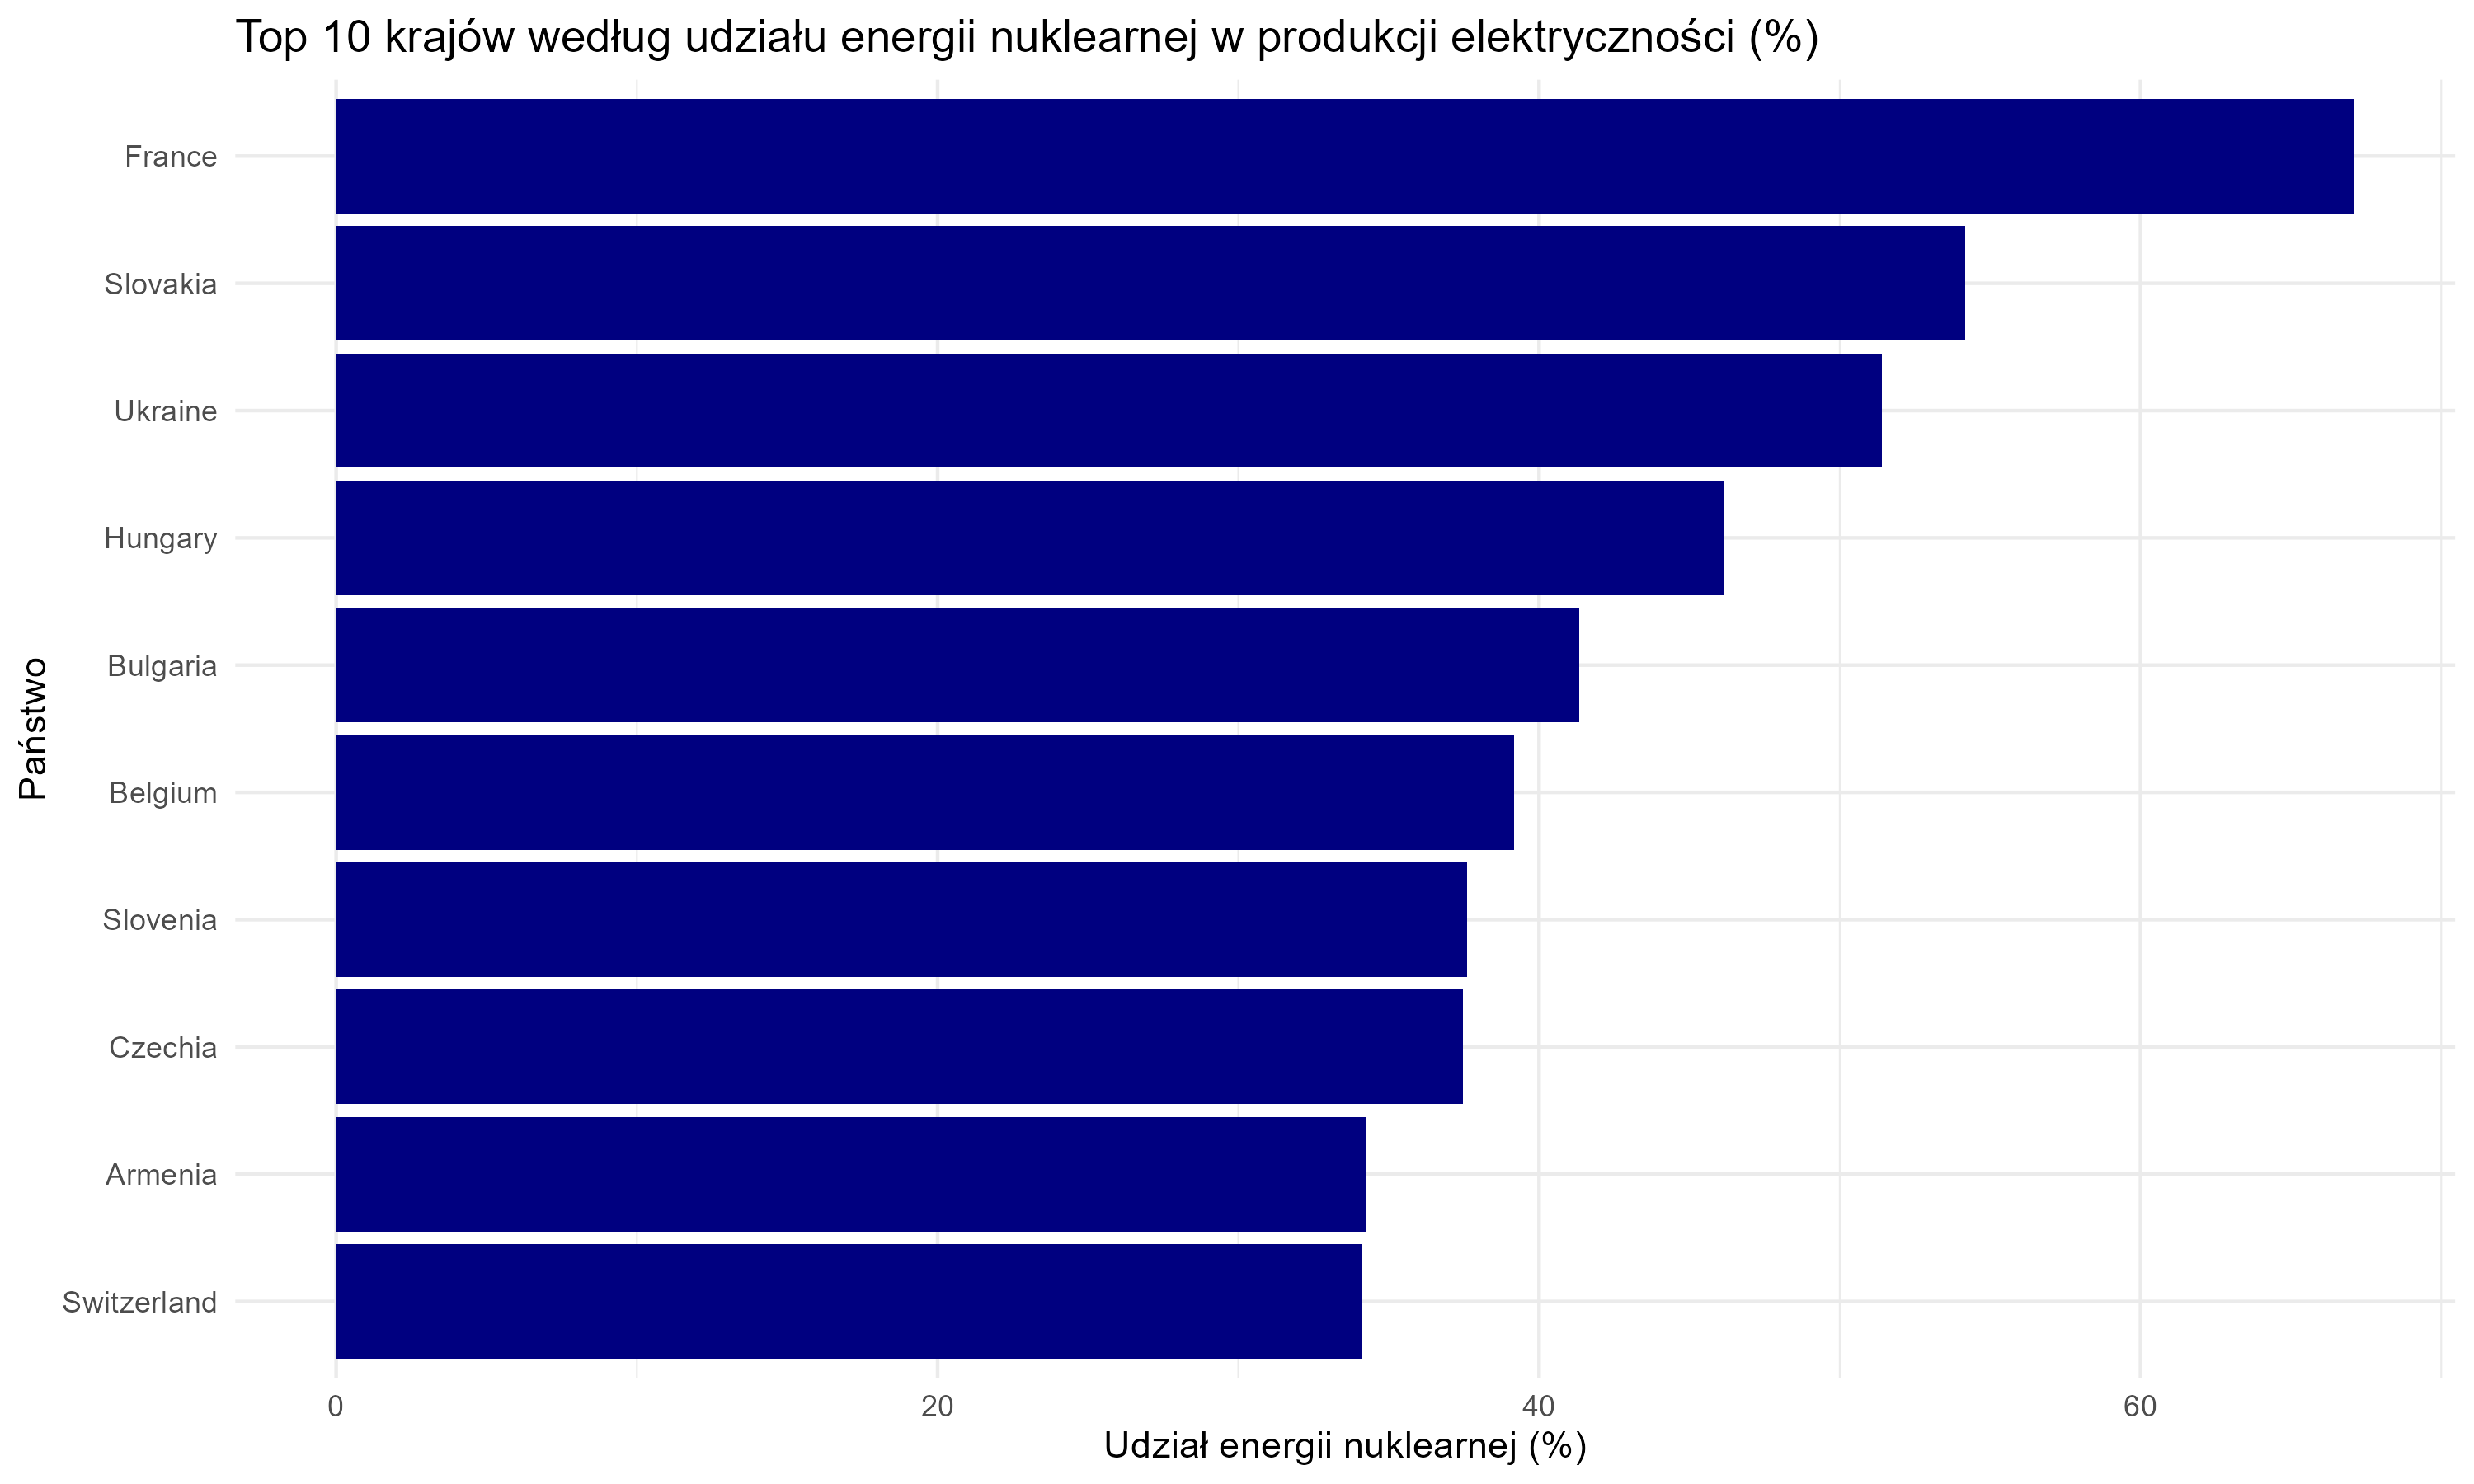
\includegraphics[width=\textwidth]{phts/4/png/11.png}
    \caption{Udział energii nuklearnej (top 10).}
\end{figure}

Największy udział energii nuklearnej mają kraje takie jak Francja, Słowacja i Ukraina. Te kraje zainwestowały znaczne środki w rozwój energetyki jądrowej.

\subsection{Wnioski}
\begin{enumerate}
    \item W latach 2000--2020 globalne emisje CO2 wzrosły pomimo rosnącego udziału odnawialnych źródeł energii (OZE). Oznacza to, że rozwój OZE nie nadążył za wzrostem zapotrzebowania energetycznego.
    \item Wyższy udział OZE koreluje ze zmniejszonymi emisjami CO2 w przeliczeniu na produkcję energii, co sugeruje, że dalsze inwestycje w OZE mogą skutecznie obniżać emisje.
    \item Produkcja energii nuklearnej spadła po awarii w Fukushimie (2011), lecz później wróciła do poziomów sprzed zdarzenia. Możliwe są też dalsze inwestycje w energię jądrową.
    \item Wiele państw o bogatych zasobach paliw kopalnych wciąż ma niski udział OZE i wysokie emisje per capita.
    \item Wsparcie polityczne i inwestycyjne jest kluczowe, aby skalować OZE i zredukować emisje w przyszłości.
\end{enumerate}






\newpage
\section{Kosmiczne śmieci - co krąży nad naszymi głowami?}

Przygotowane przez: \textbf{Jan Domański}

\subsection{Źródło danych}
\href{https://celestrak.org/pub/satcat.csv}{CelesTrak - SATCAT - Satellite Catalog}\\
\url{https://celestrak.org/pub/satcat.csv}

\href{https://celestrak.org/satcat/satcat-format.php}{Dokumentacja formatu SATCAT}\\
\url{https://celestrak.org/satcat/satcat-format.php}

\subsection{Opis zbioru i istotnych pojęć}
\begin{itemize}
    \item Dane pochodzą z katalogu SATCAT prowadzonego przez CelesTrak.
    \item Analizowany plik zawierał \textbf{69 124 rekordy} obiektów z okresu od \textbf{1957} do \textbf{2026} roku.
    \item W wizualizacjach pominięto kategorię \texttt{UNK}, czyli obiekty o nieznanym typie, ponieważ nie wnosiła żadnej informacji interpretacyjnej.
    \item Każdy rekord opisuje pojedynczy obiekt znajdujący się w katalogu, np. satelitę, człon rakiety albo fragment powstały po rozpadzie lub kolizji (po ang. debris).
    \item Najważniejsze kolumny wykorzystane w analizie to:
    \begin{itemize}
        \item \texttt{OBJECT\_NAME} - nazwa obiektu,
        \item \texttt{OBJECT\_TYPE} - typ obiektu,
        \item \texttt{OWNER} - właściciel, kraj lub organizacja odpowiedzialna za obiekt,
        \item \texttt{LAUNCH\_DATE} - data startu,
        \item \texttt{LAUNCH\_SITE} - miejsce startu,
        \item \texttt{DECAY\_DATE} - data zejścia z orbity, jeżeli obiekt już zdeorbitował,
        \item \texttt{PERIGEE} i \texttt{APOGEE} - najniższa i najwyższa wysokość orbity,
        \item \texttt{OPS\_STATUS\_CODE} - kod statusu operacyjnego.
    \end{itemize}
    \item \textbf{Satelita / payload} - ładunek wyniesiony na orbitę, np. satelita telekomunikacyjny, obserwacyjny lub naukowy.
    \item \textbf{Człon rakiety} - część rakiety, która po wyniesieniu ładunku może pozostać na orbicie.
    \item \textbf{Fragment / debris} - odłamek/pozostałość po rozpadzie, eksplozji czy kolizji czy innym zdarzeniu związanym z obiektem orbitalnym.
    \item \textbf{Obiekt nadal na orbicie} - obiekt, dla którego w danych nie występuje data zejścia z orbity.
    \item \textbf{LEO, MEO, GEO/GSO, HEO} - uproszczone klasy orbit według średniej wysokości obiektu nad ziemia.
\end{itemize}

\newpage
\subsection{Wizualizacje zbioru}

\subsubsection{Typy obiektów wysyłanych w kolejnych latach}
\begin{figure}[H]
    \centering
    
\includegraphics[width=\textwidth]{phts/5/png/5.1.png}
    \caption{Liczba obiektów wysłanych w kolejnych latach według typu obiektu.}
\end{figure}

Wykres pokazuje, że przez wiele dekad liczba wynoszonych satelitów była w miarę stabilna, a po 2020 roku nastąpił bardzo silny wzrost liczby obiektów typu payload/satelita. Fragmenty orbitalne / debris maja bardziej nieregularny przebieg, ponieważ ich liczba często rośnie skokowo po pojedynczych zdarzeniach (rozpady/kolizje na przykład) Człony rakiet występują bardziej systematycznie, ale ich liczba w jest znacznie mniejsza niż liczba satelitów i fragmentów.

\subsubsection{Narastanie katalogu obiektów orbitalnych}
\begin{figure}[H]
    \centering
    
\includegraphics[width=\textwidth]{phts/5/png/5.2.png}
    \caption{Narastanie liczby obiektów w katalogu SATCAT oraz liczby obiektów nadal pozostających na orbicie.}
\end{figure}

Wykres przedstawia różnicę między liczbą wszystkich obiektów a liczbą obiektów, które według danych wciąż są na orbicie. Obie wartości rosną w czasie, lecz całkowita liczba obiektów w katalogu jest znacznie większa, ponieważ obejmuje też te obiekty, które już zeszły z orbity. Szczególnie szybki wzrost po 2015/2020 roku pokazuje, że orbita ziemska jest coraz intensywniej wykorzystywana, a problem kosmicznych śmieci staje się coraz bardziej poważny.

\subsubsection{Struktura obiektów w katalogu SATCAT}
\begin{figure}[H]
    \centering
    
\includegraphics[width=\textwidth]{phts/5/png/5.3.png}
    \caption{Liczba i udział podstawowych typów obiektów w katalogu SATCAT.}
\end{figure}

\newpage

Największą grupę w katalogu stanowią fragmenty (debris). Odpowiadają one za ponad połowę rekordów w bazie danych. Satelity i inne ładunki użytkowe są drugą największą kategorią, a człony rakiet stanowią mniejszy, lecz wciąż istotny udział. Wykres pokazuje, że omawiany problem nie dotyczy jedynie aktywnych satelitów, lecz także dużej liczby pozostałości po wcześniejszych misjach.

\subsubsection{Kraje i organizacje z największą liczbą obiektów w katalogu}
\begin{figure}[H]
    \centering
    
\includegraphics[width=\textwidth]{phts/5/png/5.4.png}
    \caption{Właściciele, kraje i organizacje z największą liczbą obiektów w katalogu SATCAT.}
\end{figure}

Największą liczbę obiektów w katalogu mają Stany Zjednoczone, Rosja / ZSRR / WNP oraz Chiny. Wynika to z ich długiej historii aktywności kosmicznej i bardzo dużej liczby startów. Należy pamiętać, że wykres obejmuje wszystkie obiekty w zbiorze, a więc zarówno obiekty nadal znajdujące się na orbicie, jak i te, których już nie ma na orbicie.

\subsubsection{Kraje i organizacje z największą liczbą obiektów nadal na orbicie}
\begin{figure}[H]
    \centering
    
\includegraphics[width=\textwidth]{phts/5/png/5.5.png}
    \caption{Właściciele, kraje i organizacje z największą liczbą obiektów nadal pozostających na orbicie Ziemi.}
\end{figure}

Po ograniczeniu danych do obiektów nadal pozostających na orbicie zmienia się struktura rankingu. Stany Zjednoczone mają teraz największą liczbę takich obiektów (i to zdecydowanie), a Chiny i Wielka Brytania znajdują się też wysoko w rankingu. Różnica względem poprzedniego wykresu pokazuje, że historyczna liczba obiektów w zbiorze danych i aktualne obciążenie orbity nie są tym samym wskaźnikiem i się od siebie zdecydowanie różnią.

\subsubsection{Status operacyjny obiektów nadal na orbicie}
\begin{figure}[H]
    \centering
    
\includegraphics[width=\textwidth]{phts/5/png/5.6.png}
    \caption{Status operacyjny obiektów nadal pozostających na orbicie.}
\end{figure}

\newpage

Wykres pokazuje jak większość obiektów z dostępnym statusem operacyjnym jest oznaczona jako operacyjna. Widoczna jest grupa obiektów nieoperacyjnych i częściowo operacyjnych. Oznacza to, że sama obecność obiektu na orbicie nie mówi jeszcze, czy pełni funkcję użyteczną. Z punktu widzenia problemu kosmicznych śmieci ważne są głównie obiekty nieaktywne, ponieważ nadal zajmują przestrzeń na orbicie i mogą zwiększać ryzyko potencjalnych kolizji.

\subsubsection{Rozmieszczenie typów obiektów według klas orbit}
\begin{figure}[H]
    \centering
    
\includegraphics[width=\textwidth]{phts/5/png/5.7.png}
    \caption{Liczba obiektów według typu i klasy orbity.}
\end{figure}

Największa koncentracja obiektów znajduje się na niskiej orbicie okołoziemskiej czyli LEO. Dotyczy to satelitów, jak i fragmentów. MEO i GEO/GSO mają mniejsze liczby obiektów, lecz też są ważne, ponieważ pełnią istotne funkcje nawigacyjne czy komunikacyjne. Wysokie orbity HEO zawierają znacznie mniej obiektów w porównaniu np. do LEO.

\subsubsection{Ranking przedziałów wysokości orbit}
\begin{figure}[H]
    \centering
    
\includegraphics[width=\textwidth]{phts/5/png/5.8.png}
    \caption{Ranking przedziałów średniej wysokości orbity według liczby obiektów.}
\end{figure}

\newpage

Wykres jest uporządkowany według liczby obiektów, dlatego nie pokazuje naturalnej kolejności wysokości, lecz ranking tych przedziałów orbiatalnych, które sa najbardziej zatłoczone. Najwięcej obiektów znajduje się poniżej 500 km oraz w przedziale 500-800 km. Wysoko znajduje się także zakres 33 000-38 000 km, który odpowiadają obszarowi orbit geostacjonarnych. To wszystko łatwo pokazuje, które wysokości są najbardziej obciążone na orbicie.

\subsubsection{Kosmodromy z największą liczbą obiektów w katalogu}
\begin{figure}[H]
    \centering
    
\includegraphics[width=\textwidth]{phts/5/png/5.9.png}
    \caption{Kosmodromy i miejsca startu, z których pochodzi najwięcej obiektów w katalogu.}
\end{figure}

Najwięcej obiektów w katalogu powiązanych jest z największymi historycznie miejscami startu: Cape Canaveral, Plesieckiem, Vandenbergiem i Bajkonurem. Wartości na wykresie nie oznaczają liczby samych startów, tylko liczbę obiektów przypisanych do danego miejsca startu w bazie. Jeden start może bowiem wygenerować wiele obiektów.

\subsubsection{Zejścia obiektów z orbity według dekad}
\begin{figure}[H]
    \centering
    
\includegraphics[width=\textwidth]{phts/5/png/5.10.png}
    \caption{Liczba obiektów schodzących z orbity według dekady i typu obiektu.}
\end{figure}

Wykres pokazuje, w których dekadach obiekty najczęściej schodziły z orbity. Fragmenty dominują w wielu okresach. Dla satelitów szczególnie widoczny jest wzrost w latach 2020., co może być związane z większą liczbą obiektów na niskich orbitach, jak i z krótszym czasem życia części współczesnych satelitów. Człony rakiet mają bardziej stabilny rozkład.

\newpage
\subsection{Wnioski}
\begin{enumerate}
    \item Katalog SATCAT pokazuje, że liczba obiektów związanych z działalnością kosmiczną systematycznie rosła od 1957 roku, a po 2020 roku wzrost znacznie przyspieszył.
    \item Największą część katalogu stanowią fragmenty, czyli debris. Oznacza to, że kosmiczne śmieci są ilościowo większym problemem niż aktywne satelity same w sobie.
    \item Największy historyczny udział w liczbie obiektów mają Stany Zjednoczone, Rosja / ZSRR / WNP oraz Chiny, czyli państwa o największej aktywności kosmicznej.
    \item Ranking obiektów znajdujących się na orbicie nadal różni się od rankingu historycznego. Trzeba odróżniać całkowitą aktywność kosmiczną od aktualnego obciążenia orbity.
    \item Największe zagęszczenie obiektów występuje na niskiej orbicie okołoziemskiej LEO - głównie poniżej 800 km.
    \item Orbita geostacjonarna również jest istotnym obszarem koncentracji obiektów, pomimo tego iż znajduje się znacznie wyżej niż LEO.
    \item Duże kosmodromy, np. jak Cape Canaveral, odpowiadają za największą liczbę obiektów wg miejsca startu.
    \item Obiekty nieoperacyjne i częściowo operacyjne są szczególnie ważne z punktu widzenia bezpieczeństwa na orbicie, gdyż wciąż mogą zwiększać ryzyko kolizji.
    \item Problem kosmicznych śmieci nie polega tylko na liczbie satelitów, lecz także na pozostałościach po startach, członach rakiet, fragmentach powstałych po wcześniejszych zdarzeniach na orbicie.
\end{enumerate}


\section{Korzystanie z internetu w krajach UE-27}

Przygotowane przez: \textbf{Jan Machowski}

\subsection{Źródło danych}

\url{https://ec.europa.eu/eurostat/web/digital-economy-and-society/indicators/main-tables}
Tabelki - tin00028, tin00094, tin00095, tin00099, tin00101, tin00102, tin00127, tin00129.


\subsection{Opis zbioru i istotnych pojęć}

\begin{itemize}
    \item Dane pochodzą z corocznych badań Eurostatu w ramach modułu \textbf{ICT Usage in Households and by Individuals}, 
    prowadzonych w 27 krajach Unii Europejskiej;
    \item Zbiór obejmuje lata 2014-2025. Dla niektórych kategorii (bankowość internetowa, informacje zdrowotne, poszukiwanie pracy) dostępne są 
    dane od wcześniejszych edycji, jednak niniejsza analiza ogranicza się do wspólnego okna czasowego;
    \item Jednostka obserwacji – odsetek osób w wieku 16--74 lata, które korzystały z internetu w ciągu ostatnich 3 miesięcy 
    (lub podkategorie tej aktywności).

    \item W ramach wizualizacji zebrane zostały tabelki będące podzbiorami głównej metryki. Poniżej opisane są natury tych podzbiorów:
    \begin{itemize}
        \item \textbf{Ogólne korzystanie z internetu} – jakakolwiek aktywność online w ciągu ostatnich 3 miesięcy;
        \item \textbf{Wysyłanie/odbiór e-maili} – korzystanie z poczty elektronicznej;
        \item \textbf{Wyszukiwanie towarów i usług} – przeglądanie ofert zakupowych online;
        \item \textbf{Bankowość internetowa} – zarządzanie finansami przez internet oraz aplikacje komórkowe wykorzystujące internet;
        \item \textbf{Media społecznościowe} – korzystanie z portali społecznościowych;
        \item \textbf{Informacje zdrowotne} – szukanie informacji o zdrowiu oraz wykrozystywanie portali zdrowotnych online;
        \item \textbf{Poszukiwanie pracy} – używanie internetu do szukania zatrudnienia lub przeglądania otwartych pozycji;
        \item \textbf{Konsultacje / głosowanie online} – udział w konsultacjach społecznych lub e-głosowaniach, w krajach w których jest to dostępne.
    \end{itemize}

    \item Jedynym brakiem danych w całym zbiorze jest Francja w roku 2020.
\end{itemize}




\newpage
\subsection{Wizualizacje zbioru}

\subsubsection{Ogólny trend korzystania z internetu}

\begin{figure}[H]
    \includesvg[width=\textwidth]{phts/6/svg/6.1.svg}
    \caption{Odsetek osób (16-74 lata) korzystających z internetu w ciągu ostatnich 3 miesięcy – średnia UE-27 w latach 2014-2025.}
\end{figure}

Ogólne korzystanie z internetu w krajach Unii Europejskiej rośnie stabilnie, co przedstawia powyższy wykres liniowy. 
Tendencja jest znaczna - na przestrzeni 11 lat, procent użytkowników zmienił się z 76,9\% do 94\% - o niecałe 20\%, przy obiektywnie 
wysokim odsetku w roku początkowym. Wzrost jest względnie równomierny – bez nagłych skoków ani wyraźnych efektów związanych z odpowiednim rokiem.
Świadczy to o dojrzałości procesu cyfryzacji: w krajach już wysoce skomunikowanych nasycenie zbliża się do maksimum, natomiast kraje
doganiające podnoszą średnią wraz ze swoim wzrostem.




\subsubsection{Mapa cieplna intensywności korzystania z internetu}

\begin{figure}[H]
    \includesvg[width=\textwidth]{phts/6/svg/6.2.svg}
    \caption{Intensywność korzystania z internetu w UE-27 na przestrzeni lat.}
\end{figure}

Mapa cieplna porządkuje kraje według poziomu cyfryzacji: Skandynawia, Luksemburg i Holandia od pierwszego roku analizy oscylują przy granicy 100\%, 
natomiast Bułgaria i Rumunia zaczynają od poziomów poniżej 60\%. Wyraźne jest też, że dolna część rankingu zmienia kolor znacznie szybciej niż górna 
– kraje doganiające przyspieszają, co prowadzi do stopniowego wyrównywania się rozkładu w całej UE. 

Biała komórka, będąca wynikeim Francji w 2020 roku, jest jedynym brakiem w zbiorze. Nie wpływa to jednak na interpretację wyników.



\subsubsection{Ranking krajów według korzystania z internetu (2025)}

\begin{figure}[H]
    \includesvg[width=\textwidth]{phts/6/svg/6.3.svg}
    \caption{Ranking krajów UE-27 pod względem odsetka osób korzystających z internetu w 2025r.}
\end{figure}

W 2025 r. czołują Irlandia (99,8\%), Holandia i Dania (po 99,7\%), potem Luksemburg i inne kraje nienależące do bloku wschodniego w XX wieku. 
Kraje niegdyś należące do Związku Radzieckiego pojawiają się dopiero w połowie z Litwą na poziomie 94,5\%. 

Polska z wynikiem 89,7\% zajmuje 22. miejsce spośród 27 krajów. Ciekawym jest fakt, iż dystans między Polską a unijną czołówką wynosi blisko 10 pp., 
lecz, jak zobaczymy na późniejszych wykresach, widać że Polska systematycznie nadrabia zaległości sprzed lat.

Kraje na końcu stawki (Chorwacja 85,9\%, Bułgaria 86,8\%) wykazują jednak, że mimo ogólnego postępu znaczne różnice wewnątrz Unii wciąż istnieją.




\subsubsection{Przyrost korzystania z internetu 2014 - 2025}

\begin{figure}[H]
    \includesvg[width=\textwidth]{phts/6/svg/6.4.svg}
    \caption{Przyrost korzystania z internetu w latach 2014-2025 w poszczególnych krajach wyrażona w punktach procentowych.}
\end{figure}

Dynamikę wzrostu odwraca ówczesny ranking: kraje o najniższym punkcie startowym, takie jak Rumunia, Bułgaria czy Włochy,
mają największy wzrost - odpowiednio +39,1 pp., +31,4 pp., +28,4 pp. Potwierdza to teorię "efektu doganiania" krajów do standardów 
cyfryzacji pozostałej części Europy. Natomiast kraje od lat wysoce cyfrowe - Dania, Finlandia, Luksemburg, 
notują zasadniczo niskie wzrosty z prostego powodu - nie mają już praktycznie gdzie rosnąć. 

Polska z wynikiem +23,1 pp. mieści się nieco powyżej mediany. 


\subsubsection{Rozkład korzystania z internetu w UE-27}

\begin{figure}[H]
    \includesvg[width=\textwidth]{phts/6/svg/6.5.svg}
    \caption{Rozkład odsetka użytkowników internetu w 27 krajach UE na przestrzeni lat.}
\end{figure}

Wykres pudełkowy potwierdza dwie wspomniane wcześniej tendencje jednocześnie: Po pierwsze, cały rozkład przesuwa się w górę rok do roku, pokazując
całkowity wzrost wykazany na wcześniejszych wykresach. Po drugie, rozstęp międzykwartylowy systematycznie maleje, co oznacza zbieżność
krajów Unii do stałego poziomu cyfryzacji: W 2014 r. środkowa połowa krajów mieściła się w przedziale ok. 68-84\%, a w 2025 r. ten sam przedział 
zawęził się do ok. 91-97\%. 


\subsubsection{Rozkład korzystania z internetu – wykres skrzypcowy dla wybranych lat.}


\begin{figure}[H]
    \includesvg[width=\textwidth]{phts/6/svg/6.6.svg}
    \caption{Rozkład skrzypcowy korzystania z internetu w krajach, w latach 2015, 2019 i 2025.}
\end{figure}

Rozszerzając poprzednie pudełka dla wybranych lat na poczatku, w środku i na końcu osi lat o rozkład procentowy krajów ponownie ilustrowana jest
znaczna tendencja nagłego przyrostu większej liczby krajów do wysokiego stanu cyfryzacji - kraje „starodawne" i „nowożytnie" technologicznie UE 
znacznie zmieniły swoją liczbę, od bardziej wydłużonego, chudego wykresu do krótszego, ale szerszego rozkładu.
Wskazuje to na niemal zakończony proces powszechnej cyfryzacji w obszarze podstawowego dostępu do, oraz wykorzystania, internetu.



\subsubsection{Porównanie kategorii użycia internetu dla krajów, rok 2023}

\begin{figure}[H]
    \includesvg[width=\textwidth]{phts/6/svg/6.7.svg}
    \caption{Rozkład odsetka użytkowników poszczególnych kategorii internetu w badanych krajach w 2023r.}
\end{figure}

Kategorie aktywności internetowej różnią się dramatycznie zarówno poziomem, jak i rozproszeniem. Ogólne korzystanie z internetu i 
poczta elektroniczna mają medianę powyżej 80\% i wąski rozstęp – są one powszechne i jednorodne. 
Bankowość internetowa charakteryzuje się największym rozstępem międzykwartylowym spośród wszystkich kategorii, co świadczy o dużym 
zróżnicowaniu kulturowym i infrastrukturalnym podejścia do finansów online w Europie - niektóre kraje, w 2023 roku, nie miały wielkiej popularności 
dla bankowości internetowej. Konsultacje i głosowanie online utrzymują się poniżej 15\% we wszystkich krajach – klarownie, jest to usługa niszowa.

\newpage




\subsubsection{Polska – trend korzystania z internetu wg kategorii}

\begin{figure}[H]
    \includesvg[width=\textwidth]{phts/6/svg/6.8.svg}
    \caption{Polska – odsetek osób 16-74 lata korzystających z internetu w poszczególnych kategoriach na przestrzeni lat.}
\end{figure}

W Polsce wszystkie kategorie za wyjątkiem poszukiwania pracy i konsultacji online wykazują trend wzrostowy. Ogólne korzystanie z internetu 
wzrosło z ok.~67\% do 90\% - najbardziej zauważalny wzrost zanotowały media społecznościowe, wzrastając z ok. 41\% do 69\%, oraz 
wyszukiwanie towarów i usług które wzrosły z 50\% do 66\%. 

Ciekawym spostrzeżeniem jest dołek wielu kategorii w latach 2020-2021. Powodem nich może być świat pandemiczny COVID-19 lub rzeczywista zmiania 
zachowań polaków - najbardziej widocznym spadkiem jest wyszukiwanie towarów i usług, które faktycznie nie były najpopularniejszym tematem 
w czasie globalnego lock-down'u.




\subsubsection{Niemcy – trend korzystania z internetu wg kategorii}

\begin{figure}[H]
    \includesvg[width=\textwidth]{phts/6/svg/6.9.svg}
    \caption{Niemcy – odsetek osób (16--74 lata) korzystających z internetu w poszczególnych kategoriach na przestrzeni lat.}
\end{figure}

Profil kategorii w Niemczech różni się od polskiego w kilku istotnych aspektach. Po pierwsze, ogólne korzystanie z internetu i poczta elektroniczna
od lat utrzymują się powyżej 85\%. Po drugie, wyszukiwanie towarów i usług oraz informacje zdrowotne wykazują gwałtowne spadki i odbicia w
latach 2021-2023, co jest bardziej charakterystycznym znacznikiem zmian przyzwyczajeń i wprowadzonych obostrzeń podczas pandemii.

Bankowość internetowa wzrosła z ok.~49\% do 71\%, a media społecznościowe – mimo wcześniejszej rezerwy – osiągnęły w 2025 r. 
poziom zbliżony do polskiego (ok.~60\%).




\subsubsection{Polska vs Niemcy – ogólne korzystanie z internetu}

\begin{figure}[H]
    \includesvg[width=\textwidth]{phts/6/svg/6.10.svg}
    \caption{Porównanie trendu ogólnego korzystania z internetu w Polsce i Niemczech na przestrzeni lat.}
\end{figure}

Jak widać na wykresie, Niemcy na przestrzeni całego zbioru danych korzystają z internetu więcej, niż Polacy.
Dystans między Polską a Niemcami wynosił w 2014~r. blisko 20\%.

Natomiast, systematyczne nadrabianie zaległości przez Polskę, prawdopodobnie spowodowane dzięki inwestycjom infrastrukturalnym 
i rosnącej roli smartfonów, skróciło tę lukę do 5\% w 2025 r. Niemcy, mimo wyższego punktu startowego, kilkukrotnie doświadczyły 
krótkotrwałych spadków, co zanotowała również Polska.
Przy utrzymaniu obecnego tempa wzrostu Polska prawdopodobnie zrówna się z Niemcami w perspektywie 3-5 lat.




\subsubsection{Porównanie wybranych krajów wg kategorii - 2025 rok}

\begin{figure}[H]
    \includesvg[width=\textwidth]{phts/6/svg/6.11.svg}
    \caption{Porównanie 8 wybranych krajów - Polska, Niemcy, Francja, Szwecja, Bułgaria,
   Dania, Włochy, Rumunia - względem korzystania z internetu w poszczególnych kategoriach w 2025r.}
\end{figure}
  
Wykres słupkowy ujawnia wyraźne narodowe wzorce korzystania z internetu. Na najwyższych poziomach w każdej kategorii jest Dania - jej bankowość
internetowa jest ponad półtora raza wyższa niż w Polsce czy Rumunii.

Bułgaria i Rumunia odstają, w negatywny sposób, w dwóch charakterystycznych kategoriach - bankowości i wyszukiwaniu towarów. 
Widać, że ludzie w tych krajach nadal są przyzwyczajeni do starodawnych metod - sklepów lub targów / marketów naziemnych, natomiast 
w kategorii mediów społecznościowych są bardzo blisko pozostałych krajów.

Polska wyróżnia się relatywnie niskim wskaźnikiem poszukiwania pracy online - niecałe 9\%, poza czym jest 
bardzo bliska medianie.

Obiektywnie najgorsza integracyjnie kategoria to konsultacje/głosowanie online - jest to kategoria o zarówno najmniejszym zróżnicowaniu krajowym
i najniższych bezwzględnych wartościach (2--14\%) w całej próbie.

\newpage




\subsubsection{Bankowość vs Media społecznościowe – wybrane kraje}

\begin{figure}[H]
    \includesvg[width=\textwidth]{phts/6/svg/6.12.svg}
    \caption{Porównanie trendów bankowości internetowej i mediów społecznościowych dla 8 wybranych krajów na przestrzeni lat.}
\end{figure}

Zestawienie dwóch oddzielnych ideowo kategorii - bankowości i mediów społecznościowych - ujawnia ciekawy przykład różnicy różnorodności wartości, 
ale tej samej tendencji kategorycznej dla krajów Unii Europejskiej.
Obie z tych kategorii stopniowo rosną, lecz zróżnicowanie między krajami w bankowości internetowej jest ogromne i utrzymuje się przez cały badany okres:
Dania oscyluje najwyżej, podczas gdy Bułgaria i Rumunia startowały praktycznie przy zerze i doszły do ok. 30\%. W przeciwieństwie, media społecznościowe 
przedstawiają historię gdzie kraje "doganiające" rosły szybciej, co doprowadziło do znacznego wyrównania poziomu: w 2025~r. większość krajów znajduje się
w przedziale 60-90\%. Polaryzacja jest zatem wyraźniejsza w bankowości niż w mediach społecznościowych, jednak tendencja wzrostowa utrzymuje się 
niezależnie od kategorii.




\subsubsection{Bankowość internetowa vs Media społecznościowe w UE-27 (2025) – scatter}

\begin{figure}[H]
    \includesvg[width=\textwidth]{phts/6/svg/6.13.svg}
    \caption{Wykres rozrzutu: bankowość internetowa a media społecznościowe w 27 krajach UE w 2025~r.}
\end{figure}

Korzystając z porónania poprzednich aspektów wykorzystania internetu, współzależność między bankowością a mediami społecznościowymi jest
umiarkowanie dodatnia - oznacza to, ze obie z tych kategorii wzrastają, podtrzymując hipotezę z poprzedniego podrozdziału.
Istnieją jednak wyraźne, wczesniej wspomniane wyjątki. Rumunia i Bułgaria posiadają relatywnie wysoki udział mediów społecznościowych
przy bardzo niskiej bankowości internetowej – sugeruje to, że dostęp do smartfona i portali społecznościowych wyprzedza dojrzałość cyfrową
w zakresie e-finansów.
Niemcy i Włochy leżą poniżej linii trendu: wysoka bankowość przy niższych niż spodziewane wynikach mediów społecznościowych związane są
prawdopodobnie z kulturową rezerwą wobec portali społecznościowych wśród większości populacji tych krajów. Polska plasuje się przy linii trendu,
bez wyraźnych odchyleń.

\newpage



\subsubsection{Polska – korzystanie z internetu wg kategorii w wybranych latach}

\begin{figure}[H]
    \includesvg[width=\textwidth]{phts/6/svg/6.15.svg}
    \caption{Polska – korzystanie z internetu wg kategorii w czterech latach - 2015, 2018, 2021 i 2025.}
\end{figure}

Cztery przekroje czasowe dla Polski pokazują nierównomierność tempa wzrostu w odpowiednich kategoriach. Ogólne korzystanie z internetu wzrosło, 
co zostało przekazane w większości poprzednich wykresów, i jest dominującą wartością - co ma sens, gdyż korzystanie z internetu w dowolnym 
celu należy do korzystania z internetu. Najmniejszymi wykorzystaniami na przestrzeni lat są wyszukiwanie pracy oraz konsultacje / głosowanie online.
Ciekawą tendencją jest fakt, iż konsultacje wzrastają od początkowego roku - popularność i przydatność telewizyt w Polsce widocznie wzrasta, i mimo 
większościowej tendencji do korzystania ze starodawnych metod zaczyna się widać falę przejściową.




\subsubsection{Poszukiwanie pracy online – wybrane kraje}

\begin{figure}[H]
    \includesvg[width=\textwidth]{phts/6/svg/6.16.svg}
    \caption{Odsetek osób poszukujących pracy przez internet w 8 wybranych krajach - Polska, Niemcy, Francja, Szwecja, Bułgaria, Dania, Włochy, Rumunia -
                na przestrzeni lat.}
\end{figure}

Korzystając z jednej z najmniej popularnych usług wykorzystywanych w internecie, mianowicie poszukiwania pracy online, jesteśmy w stanie zwizualizować
nie tylko najniższy ale i najbardziej zmienny trendów spośród badanych kategorii. Dania i Szwecja konsekwentnie prowadzą, co może wynikać z 
elastyczności tamtejszych rynków pracy i popularności dedykowanych platform rekrutacyjnych w porównaniu z klasycznymi metodami.
Polska i Rumunia należą do najmniej aktywnych krajów w tej kategorii, mimo że ich ogólny poziom cyfryzacji jest porównywalny z resztą Unii Europejskiej
w roku 2025 - widać, że w sektorze prac, w tych krajach dalej szanuje się najprostsze sposoby rozmowy o pracę i składania papierowych CV.





\subsubsection{Wzrost bankowości internetowej}

\begin{figure}[H]
    \includesvg[width=\textwidth]{phts/6/svg/6.18.svg}
    \caption{Przyrost odsetka użytkowników bankowości internetowej na przestzeni lat w badanych krajach.}
\end{figure}


Bankowość internetowa to kategoria o największej bezwzględnej dynamice wzrostu w całej analizie. Liderami przyrostu są, zaskakująco, Cypr, Grecja
Irlandia oraz Chorwacja. Są to kraje, które jeszcze w 2014 r. miały bardzo niski punkt startowy i w następnej dekadzie nadrabiały zaległości,
napędzane rozwojem bankowości mobilnej. Polska znajduje się poniżej mediany wzrostu, co może wydawać się zaskakujące biorąc pod uwagę dynamiczny
rozwój polskiego sektora fintech z technologiami takimi jak BLIK czy aplikacjami mobilnymi banków. Wynika to jednak z faktu, że w Polsce poziom
bazowy z 2014 r. był wyższy niż we wcześniej wspomnainych krajach. Szwecja była od początku niemal w pełni nasycona, więc jej najniższy wzrost jest 
spodziewany.


\newpage
\subsection{Wnioski}

\begin{enumerate}
    \item Korzystanie z internetu w Unii Europejskiej wzrosło między 2014 a 2025 r. z 76,9\% do 94\% – niemal monotonicznie i bez skokowych 
    efektów pandemicznych na poziomie średniej unijnej;
    \item Konwergencja cyfrowa postępuje: rozstęp między krajami maleje rok do roku, co potwierdzają zarówno analiza wykresu pudełkowego,
    jak i zmiana kształtu skrzypiec z bimodalnego (2015) na skupiony (2025);
    \item Polska z wynikiem 89,7\% w 2025~r. zajmuje 22. pozycję spośród 27 krajów, lecz jej wzrost o 23,1\%. od 2014~r. klasyfikuje ją w górnej
    połowie stawki pod względem dynamiki. Polacy wyraźnie doganianiają resztę europejczyków;
    \item Dystans między Polską a Niemcami skurczył się z ok.~20\%. w 2014 r. do ok. 5\% w 2025~r., co wskazuje na możliwe wyrównanie w
    perspektywie kilku następnych lat;
    \item Kategorie aktywności internetowej różnią się dramatycznie: poczta e-mail i bankowość mają powyżej 80\% mediany w UE,
    natomiast konsultacje i głosowanie online nie przekraczają 15\% w żadnym kraju, co świadczy o słabości e-demokracji w Europie.
    \item Bankowość internetowa to kategoria o największej bezwzględnej dynamice wzrostu (+29,3\%. średnia wzrostu, lider Cypr +53,9 \%);
    \item Podziały kulturowe i ekonomiczne wewnątrz UE są wyraźniejsze w bankowości internetowej i poszukiwaniu pracy online niż w 
    mediach społecznościowych, które wykazują szybsze zbliżenie się między krajami.
\end{enumerate}


\end{document}
